ARM big.LITTLE systems are everywhere from smart devices, to Systems on Chips, 
to mobile phones. Common to these is an often limited energy budget, where 
saving energy without sacrificing too much performance. With asymmetric 
multicore processors and DVFS comes the potential for vast energy savings by 
having the scheduler be aware of the energy used by the system tasks and 
adjusting the DVFS points accordingly, potentially even switching some cores 
off entirely.

In this project, I explore these points using the gem5 Simulator, a highly 
accurate simulator with support for both DVFS and power modelling. I present 
initial findings which suggest that the use of ARM PMUs for energy prediction 
can be highly effective and accurate for scheduling, motivating further research
into the topic.

\begin{figure}[H]
    \centering
    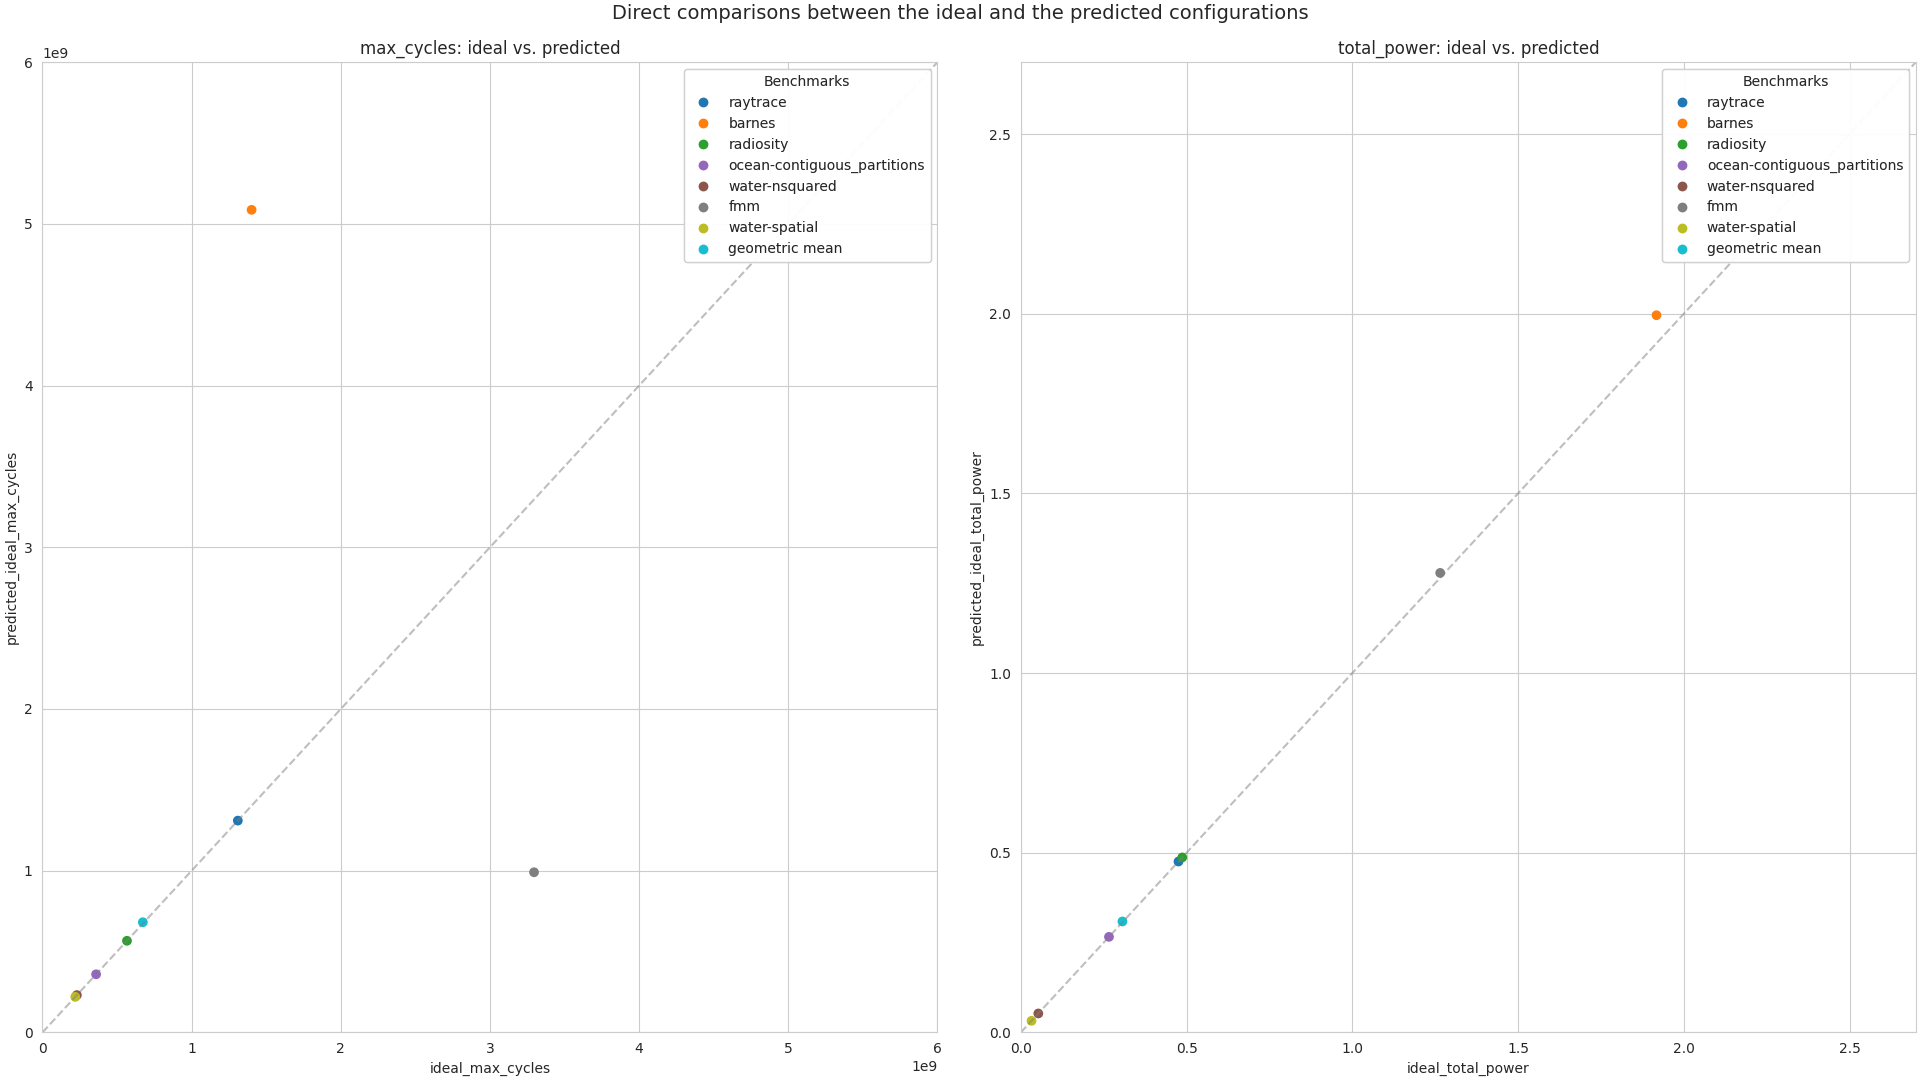
\includegraphics[width=0.6\textwidth]{result-plots/stock-2b2L/system-scatter.png}
    \caption{Initial findings encourage looking into the use of ARM PMUs in
             scheduling, in order to balance performance and energy savings}
\end{figure}
\begin{figure}[H]
    \centering
    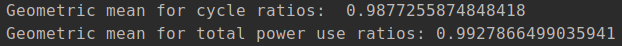
\includegraphics[width=0.6\textwidth]{screenshots/promising-geomeans.png}
    \caption{Albeit based on a small sample size, the model seems to have narrow
             optimisation space, which is promising for future research}
\end{figure}
